\chapter{Procesamiento de lenguaje natural}
El procesamiento de lenguaje natural se ocupa de la interpretación, análisis y manipulación de los lenguajes naturales por sistemas informáticos. Los lenguajes naturales presentan retos únicos. No solo son inherentemente ambiguos y se resisten a ser descritos formalmente, sino que la mayoría de problemas de lenguaje natural no están bien definidos y admiten múltiples soluciones. Desde el nacimiento de las inteligencias artificiales se ha reconocido lo importante y desafiante del campo, hasta tal punto que Alan Turing cifró la inteligencia de una máquina en su capacidad para comunicarse en lenguaje natural como lo haría un humano \cite{turing2009computing}.

La evolución del campo ha sido extremadamente rápida durante las dos últimas décadas y no ha hecho sino acelerarse con la aparición de los \textit{transformer}. En las páginas de este capítulo, tratamos de esbozar los desarrollos más significativos del campo y presentamos estrategias ya clásicas para diseñar redes neuronales para el procesamiento de lenguaje natural. 

\section{El estado de la cuestión}
\begin{figure}[tb]
    \centering
    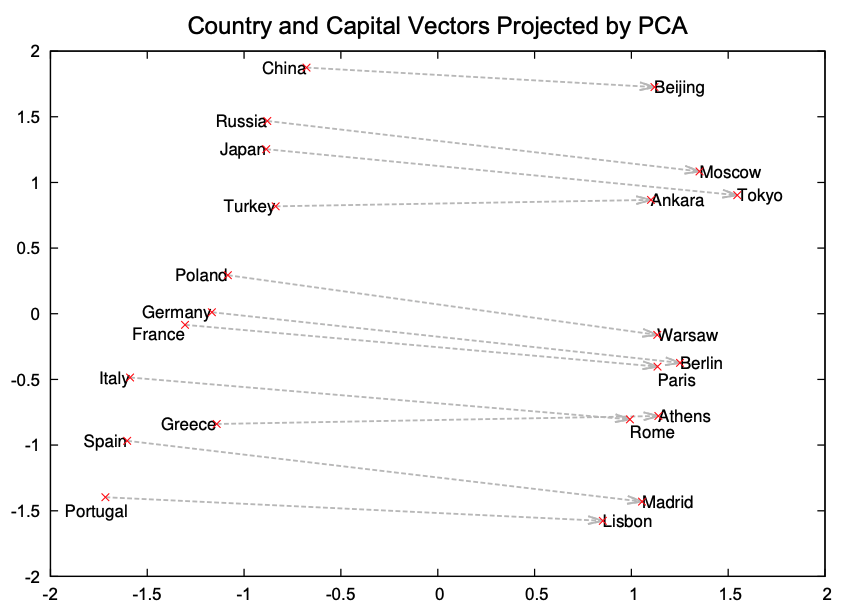
\includegraphics[width=.6\textwidth]{figures/chapter3/embeddings.png}
    \caption{Proyección a \( \real{2} \) (usando \textit{análisis de componentes principales}) de la representación generada para nombres de países y sus capitales \cite{mikolov2013distributed}. Aunque la red neuronal no tiene ninguna información sobre el concepto de ciudad capital, la representación creada por la red neuronal contiene implícitamente esta relación.}
    \label{fig:embeddings}
\end{figure}

La forma habitual de abordar los problemas de procesamiento de lenguaje natural desde las ciencias de la computación ha sido crear modelos para predecir la posibilidad de aparición de un símbolo en una secuencia a partir de los anteriores, llamados \textit{modelos de lenguaje}. La propuesta de utilizar redes neuronales para implementar modelos de lenguaje se presenta por primera vez en 2001, en un artículo extremadamente influyente \cite{bengio2000neural}. 

Tras varios intentos por encontrar una forma adecuada de manipular secuencias de longitud variable (incluyendo el uso de las convoluciones, muy comunes en los problemas de visión por ordenador \cite{collobert2011natural}), en 2014 se introducen las arquitecturas codificador-decodificador, que siguen gobernando el campo hasta la fecha \cite{sutskever2014sequence}.

En estas arquitecturas se distinguen dos componentes: el \textit{codificador}, que codifica la secuencia de entrada de longitud variable en un \textit{estado}, una representación de la entrada de longitud fija y el \textit{decodificador}, que predice la probabilidad de cada símbolo de salida a partir del estado y los símbolos ya generados.

Aunque elegante y generalizable, la arquitectura codificador-decodificador adolece de un grave problema: cuando la secuencia de entrada es larga, el contexto se vuelve incapaz de comprimir adecuadamente la información presente en dicha secuencia, deteriorando el rendimiento de la red. En un trabajo que sería el antecesor directo de las arquitecturas \textit{transformer}, un grupo de investigadores propuso que el codificador generara una secuencia de estados y el decodificador crease la salida a partir de un subconjunto de los mismos, elegidos adaptativamente usando una versión preliminar del mecanismo de atención \cite{bahdanau2014neural}. Esta estrategia evitaba el deterioro de la precisión del modelo al recibir secuencias largas y abordaba de forma elegante el problema de cómo consumir la secuencia de entrada según se genera la salida.

Alrededor del mismo tiempo aparece la propuesta de utilizar representaciones vectoriales densas (\textit{embeddings}) para codificar los símbolos de la entrada \cite{mikolov2013distributed}. En lugar de utilizar una codificación \textit{one-hot}\footnote{En la codificación \textit{one-hot} cada uno de las \( k \) símbolos es representado por un vector de la base canónica de \( \real{k} \). Se trata de una codificación \textit{dispersa}, pues cada símbolo está representado por un vector con una única componente no nula.} para representar cada símbolo, se permite que la red aprenda una representación de cada símbolo como un vector real en un espacio de dimensión prefijada (el espacio latente). Esta representación  codifica de forma espacial relaciones semánticas, como muestra la \cref{fig:embeddings}. 

\subsection{La aparición de los \textit{transformer}}
El \textit{transformer}, introducido en 2017 \cite{vaswani2017attention}, incorporaba por primera vez estas tres ideas (las representaciones densas, la arquitectura codificador-decodificador y el uso de la atención) en una red secuencial, prescindiendo tanto de la recurrencia como de las convoluciones. 

Se resolvía así uno de los grandes problemas que había acompañado a los modelos para el procesamiento de lenguaje natural: su dependencia en redes recurrentes, extremadamente profundas y con relativamente pocos parámetros, que las hacía muy vulnerables a inestabilidades numéricas, complicadas de entrenar y poco escalables.

La aparición de los \textit{transformer} generó una auténtica revolución en un campo que ya tenía una intensa actividad investigadora. Por una parte, aparecieron dos grupos de modelos muy influyentes, basados en utilizar únicamente bloques de tipo codificador o decodificador. En el primer grupo, destaca BERT \cite{devlin2018bert}, un modelo de tipo codificador que utiliza atención bidireccional (los símbolos se relacionan usando la atención con los anteriores y los siguientes) para generar representaciones con gran información de contexto. 

En el segundo grupo, el referente es la familia GPT, iniciada con GPT-1 \cite{radford2018improving} y continuada con GPT-2 \cite{gpt2trained}, GPT-3 \cite{brown2020language} y GPT-4 \cite{gpt-4}. Todos los modelos GPT tienen una arquitectura muy similar, aunque la escala de los modelos ha aumentado enormemente entre generaciones, pasando de los 117 millones de parámetros de GPT-1 a los 175.000 millones de GPT-3. Dado que era imposible crear corpus etiquetados para entrenar estos modelos de forma supervisada, estos modelos fueron pre-entrenados de forma no supervisada sobre grandes conjuntos de texto y luego afinados (\textit{fine-tuning}) para realizar tareas concretas.

En este proceso de ampliación exponencial en el número de parámetros fueron instrumentales dos importantes descubrimientos. Primero, que es posible utilizar parámetros de precisión reducida (4, 8 o 16 bits) o incluso enteros para limitar sensiblemente el tamaño de los modelos y mejorar su rendimiento \cite{wu2020integer}. Segundo, que para afinar el modelo pre-entrenado es posible congelar los parámetros del modelo (de forma que no se actualicen) y entrenar en su lugar matrices de reducción de rango con una dimensión mucho menor, una técnica llamada \textit{low-rank adaptation} \cite{hu2021lora}.

La imposibilidad de aumentar el número de parámetros de los modelos \textit{ad infinitum}, llevó a los investigadores a buscar estrategias de escalado para obtener modelos con un buen compromiso entre rendimiento y escala. El resultado fue Chinchilla \cite{hoffmann2022training}, un modelo con 70.000 millones de parámetros que superaba a modelos mucho más grandes (incluyendo a GPT-3), mediante la técnica de escalar uniformemente el tamaño del modelo y el tamaño del conjunto de entrenamiento. 

Los resultados de esta investigación fueron aplicados por los investigadores de Meta para crear LLaMA \cite{touvron2023llama}, una familia de modelos muy eficientes con un rendimiento excelente. La popularidad de LLaMA deja ver con claridad que la prioridad de los investigadores ya no es la mera creación de modelos cada vez más grandes, sino que existe una preocupación genuina por crear modelos eficientes, replicables (LLaMa ha sido íntegramente entrenado sobre conjuntos de datos públicos) y alineados.

Los anteriores párrafos solo cubren una parte muy pequeña de un campo que avanza a una velocidad francamente frenética. Por poner un ejemplo, solo entre enero y mayo del año 2023 se han establecido 16 nuevos récords en rendimiento en el conjunto de datos \textit{ScienceQA}, con preguntas y respuestas sobre ciencia.

\subsection{Grandes modelos de lenguaje}
La carrera por crear modelos \textit{transformer} cada vez de mayor escala se basa en una observación empírica: a diferencia de otras arquitecturas, los \textit{transformer} se vuelven más precisos conforme aumenta la escala del modelo. Las estimaciones empíricas apuntan a que la precisión de estas redes escala según una ley potencial con el número de parámetros, el tamaño del conjunto de datos de entrenamiento y la cantidad de recursos computacionales usados durante el entrenamiento \cite{kaplan2020scaling}, sin que sean necesarias adaptaciones significativas en el diseño de la red. Los modelos más grandes no sólo son más precisos una vez entrenados, sino que pueden alcanzar los mismos resultados que modelos más pequeños a partir de un conjunto de entrenamiento sensiblemente menor.

Lo que resulta aún más significativo es que, una vez que alcanzan una escala suficiente, estos modelos desarrollan capacidades para las que no han sido expresamente entrenados, como resolver exámenes universitarios o realizar operaciones aritméticas encadenadas \cite{wei2022emergent}. Estas capacidades se denominan \textit{habilidades emergentes} dado que no pueden extrapolarse del comportamiento de modelos más pequeños, sino que responden a un cambio cualitativo en el comportamiento del modelo derivado de cambios cuantitativos en su escala. Este cambio cualitativo tiene una naturaleza global: como muestra la \cref{fig:emergent}, habilidades muy distintas aparecen simultáneamente una vez que los modelos alcanzan una escala determinada.

\begin{figure}[tb]
    \centering
    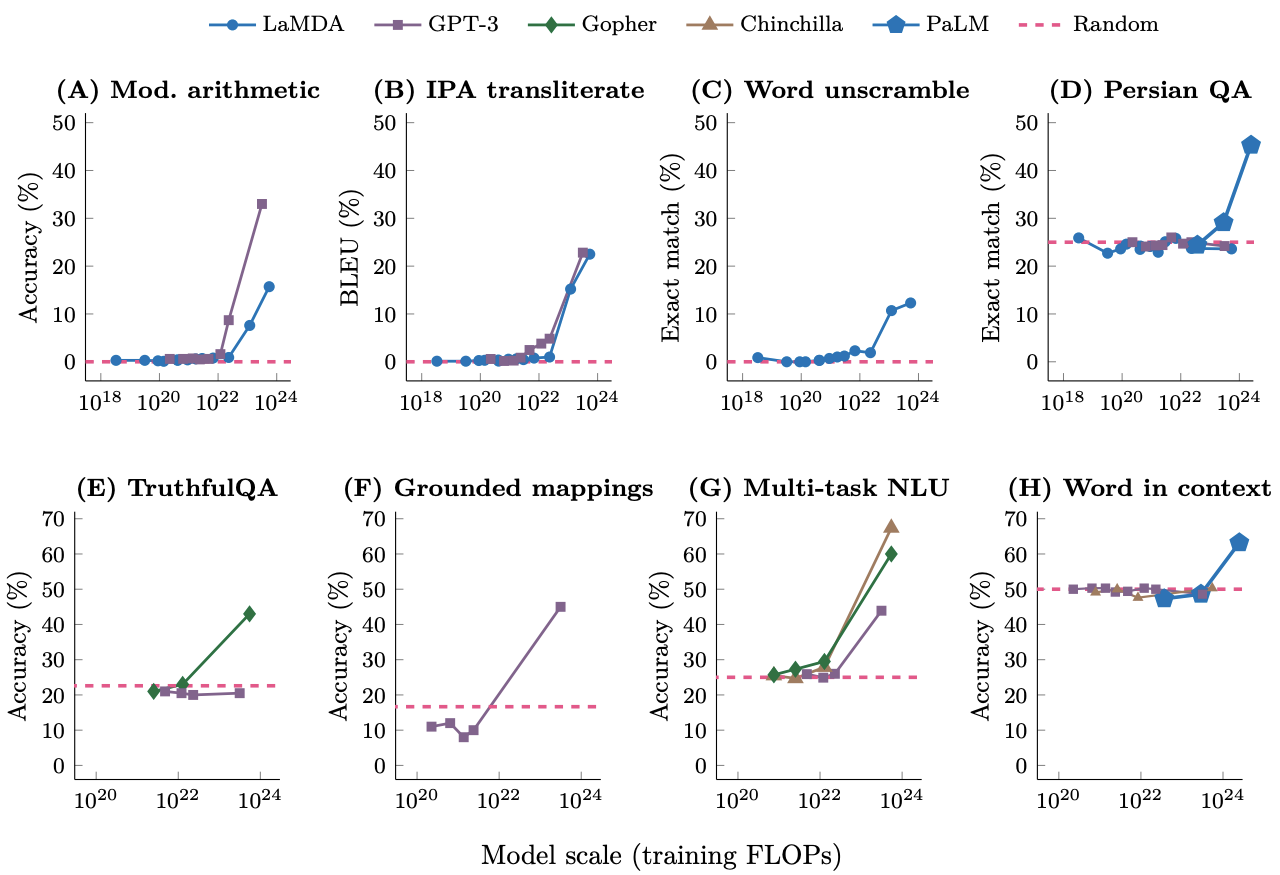
\includegraphics[width=\textwidth]{figures/chapter3/emergent.png}
    \caption{Aparición de habilidades emergentes en distintos modelos \textit{transformer} al aumentar la escala del modelo (medida en operaciones de punto flotante por segundo durante el entrenamiento) \cite{wei2022emergent}}
    \label{fig:emergent}
\end{figure}

La existencia de un comportamiento cualitativo diferencial en los modelos \textit{transformer} suficientemente grandes, ha llevado a englobar estos modelos bajo la difusa etiqueta de \textit{grandes modelos del lenguaje}. Entre los comportamientos más destacables de estos modelos, se encuentra su capacidad de aprender a realizar una nueva tarea a partir de mostrarles ejemplos resueltos, incluso cuando los parámetros se han congelado; técnica que recibe el nombre de \textit{few-shot learning}. Aunque existe todavía debate sobre cómo funciona este proceso \cite{xie2021explanation,dai2022can}, esta técnica se ha demostrado capaz de lograr resultados superiores a los de modelos específicamente afinados en multitud de tareas, como la traducción o la respuesta a preguntas \cite{brown2020language}.

También es destacable que estos modelos se han demostrado capaces de aprender a utilizar herramientas en la forma de API (interfaces de programación de aplicaciones), como motores de búsqueda, diccionarios o calculadoras \cite{schick2023toolformer}.

\subsection{Retos de los grandes modelos de lenguaje}
Los grandes modelos de lenguaje presentan retos únicos. Uno de los más fundamentales es el \textit{problema de alineamiento}: conseguir que el comportamiento de estos modelos se ajuste a los objetivos, preferencias y principios éticos de los seres humanos. Por ejemplo, un modelo no debería hacer pasar por verdaderas afirmaciones que considere falsas o generar código que contenga vulnerabilidades de seguridad.

Se trata de un problema significativo, fundamentalmente porque los objetivos humanos son complejos y pueden ser difíciles de definir. Encontrar desviaciones en el comportamiento del modelo requiere hacer pruebas extensivas y es muy complicado en los campos en los que el rendimiento de los modelos es superior al de los humanos. Las técnicas actuales de entrenamiento, que utilizan inmensos corpus de datos no supervisados sobre los que los creadores tienen poco control, hacen especialmente difícil asegurar el buen comportamiento de los modelos.

Un problema relacionado con el del alineamiento es el de la \textit{confiabilidad}. Se ha demostrado que los grandes modelos de lenguaje generan afirmaciones convincentes que son falsas y que no están sustentadas por ningún dato en el conjunto de entrenamiento, proceso conocido como \textit{alucinación} \cite{gpthallucination}. El proceso por el que se generan las alucinaciones, que han sido identificadas como uno de los principales problemas de los grandes modelos de lenguaje, es escasamente comprendido, lo que hace que estemos lejos de mitigarlas.

De hecho, la incapacidad de los modelos de lenguaje actuales para mantener un conjunto estable de creencias en el tiempo, hace imposible distinguir si las alucinaciones son un problema de \textit{deshonestidad} (el sistema hace una afirmación que sabe que es falsa) o de mera falta de \textit{confiabilidad} (el sistema hace afirmaciones que considera ciertas, aunque son incorrectas).

\section{Modelos de lenguaje}
Como ya se ha dicho, la arquitectura \textit{tranformer} es una forma de implementar \textit{modelos de lenguaje}. La definición de estos conceptos es deliberadamente amplia.

\begin{definition}[Lenguaje]
    Sea un conjunto indexado \( \mathbb{V} \) finito, que llamaremos alfabeto, y \( \mathbb{V}^* \) el conjunto de todas las sucesiones finitas de elementos de \( \mathbb{V} \). Llamamos \textit{lenguaje} a un espacio de probabilidad \( (\mathbb{V}^*, \mathbb{P}) \). A los elementos de \( \mathbb{V} \) los denominamos \textit{símbolos}, mientras que a los elementos de  \( \mathbb{V}^* \) los denominamos \textit{secuencias}.
\end{definition}

\begin{definition}[Modelo de lenguaje]
    Dado un lenguaje \( (\mathbb{V}^*, \mathbb{P}) \) llamamos \textit{modelo de lenguaje} de \( \mathbb{V^*} \) a cualquier función \( \widehat{\mathbb{P}} \), tal que \( (\mathbb{V}^*,  \widehat{\mathbb{P}}) \) es un espacio de probabilidad\footnote{Al igual que en la sección anterior, cuando el modelo de lenguaje se implemente mediante una red neuronal con parámetros \( \theta \), utilizaremos la notación \( \widehat{P}(\smallbullet; \theta) \) para subrayar la dependencia de la función calculada de los parámetros de la red.}.
\end{definition}

Habitualmente estamos interesados en aquellos modelos de lenguaje que aproximan la distribución \( \mathbb{P} \). Para ello, dada una secuencia \( x = (x_1, x_2, …, x_k) \in \mathbb{V}^* \) se explota la relación
\[
    \mathbb{P}(x) = \mathbb{P}(x_1) \mathbb{P}(x_2 \mid x_1) \ldots \mathbb{P}(x_k \mid x_1 \ldots x_{k-1})
\]
con lo que el objetivo es encontrar un modelo de lenguaje \( \widehat{\mathbb{P}} \) capaz de predecir la probabilidad de cada símbolo de una secuencia a partir de los anteriores. 

Un modelo \textit{transformer} sólo puede procesar secuencias de una determinada longitud y no tiene forma de almacenar información sobre el contenido de secuencias procesadas anteriormente, lo que hace que esté limitado al cómputo de modelos de lenguaje con una determinada \textit{longitud de contexto}.

\begin{definition}[Modelo de lenguaje con longitud de contexto]
    Sea  \( (\mathbb{V}^*, \mathbb{P}) \) un lenguaje y \( \widehat{P}(\smallbullet; \theta) \) un modelo de lenguaje de \( \mathbb{V}^* \). Decimos que \( \widehat{P} \) es un modelo de lenguaje con longitud de contexto \( l_\text{máx} \in \nat \) si para toda secuencia \( x \) de \( \mathbb{V}^* \) y toda elección de parámetros \( \theta \) se verifica:
    \begin{equation}\label{eq:prob}
        \widehat{\mathbb{P}} \left( x_{k+1} \mid  x_1, …, x_k; \theta \right) = \widehat{\mathbb{P}} \left( x_{k+1} \mid x_{k - l_\text{máx}}, …, x_k; \theta \right) \quad \text{ para todo \(k \in \nat\)}
    \end{equation}
\end{definition}

\subsection{Arquitectura codificador-decodificador}
El \textit{transformer} está diseñado para abordar problemas de \textit{secuencia a secuencia}, en los que trabajamos con dos secuencias de longitud variable. En estos casos, el lenguaje es de la forma \( ((\mathbb{V} × \mathbb{V})^*, \mathbb{P}) \) para un cierto alfabeto \( \mathbb{V} \) y el objetivo es estimar la distribución \( \mathbb{P}(x | z) \) para cada par de secuencias \( (z, x) \in \mathbb{V}^* × \mathbb{V}^* \), que reciben el nombre de \textit{contexto} y \textit{entrada} respectivamente\footnote{Por poner un ejemplo práctico, en la traducción de un texto, el contexto sería el texto en el idioma original y la entrada sería el texto ya traducido.}. 

En el caso de utilizar modelos de lenguaje limitados a una cierta longitud de contexto (el caso más habitual cuando se trabaja con redes neuronales), el modelo de lenguaje \( \widehat{P} \) verifica:
\[
    \widehat{\mathbb{P}} \left( x_{k+1} \mid  x_1, …, x_k, z \right) = \widehat{\mathbb{P}} \left( x_{k+1} \mid x_{k - l_\text{máx}}, …, x_k; z_{\phi(z; x, k+1)}, …, z_{\phi(z; x, k+1) + l_\text{máx}} \right) 
\]
para una cierta función \( \phi : \mathbb{V}^* × \mathbb{V}^* × \nat \to \nat \). El problema de elegir la función \( \phi \) se denomina problema de \textit{alineación de secuencias}, dado que es equivalente a decidir cómo se ``consume'' el contexto para generar la entrada. Este es un problema muy complejo, pues no suele existir una relación fija entre los símbolos del contexto y la entrada (por ejemplo, una palabra puede carecer de un término equivalente en otro idioma, con lo que su traducción requiere de la combinación de varios términos).

La forma predominante de abordar el problema de \textit{alineación de secuencias} es utilizar arquitecturas codificador-decodificador. 

\begin{definition}[Arquitectura codificador-decodificador]
    Sea  \( ((\mathbb{V} × \mathbb{V})^*, \mathbb{P}) \) un lenguaje. Decimos que un modelo de lenguaje tiene arquitectura codificador-decodificador si existen funciones \( c, d \) con \( c \) de la forma \( c(\smallbullet; \theta) : \mathbb{V}^* \to \real{k} \) de forma que la función \( \widehat{P} \) computada por el modelo puede escribirse como:
    \begin{equation}\label{eq:encoder}
        \widehat{P}(x \mid z; \theta) = d(x, c(z; \theta); \theta) 
    \end{equation}
    para cada \( (z, x) \in (\mathbb{V} × \mathbb{V})^* \). Las funciones \( c, d \) reciben el nombre de codificador y decodificador respectivamente.
\end{definition}

La salida del codificador, llamada \textit{estado}, genera un ``resumen'' de la información presente en el contexto, que es utilizada por el decodificador para predecir la probabilidad del próximo símbolo de la secuencia. Al eliminar la dependencia directa del decodificador sobre la secuencia de contexto, estos modelos pueden entrenarse muy eficazmente y se puede delegar en el proceso de entrenamiento la solución al problema de alineamiento de secuencias.

Antes de la aparición de los \textit{transformer}, lo habitual es que tanto codificador como decodificador se implementaran usando una red recurrente y se calculase una sucesión de estados \( \Set{h_t} \) de la misma longitud del contexto, definida recursivamente de la forma:
\begin{equation}\label{eq:rnn}
    h_t = c(z_t, h_{t-1}; \theta)
\end{equation}
a partir de la cual el decodificador computa la salida de la red.

Además de la dependencia en las redes recurrentes, cuyas inconveniencias ya hemos comentado, esta estrategia tiene un problema fundamental: conforme aumenta la longitud de la secuencia de contexto se vuelve progresivamente más difícil ``comprimir'' toda la información necesaria en el estado, lo que limita la capacidad de la red para recordar dependencias de larga longitud. Además, la dependencia entre los \( h_t \) impide que los cálculos puedan paralelizarse. 

Como veremos más adelante, la clave de los \textit{transformer} es precisamente la capacidad de adaptar las arquitecturas secuenciales, más fiables y eficientes, para abordar problemas de secuencias mediante el uso del mecanismo de atención, aplicando, ya directamente o de forma adaptada, muchas de las técnicas anteriormente utilizadas en el contexto de las redes recurrentes. 

\section{De secuencias a vectores: \textit{tokenización}}
Como hemos discutido anteriormente, las redes neuronales no trabajan directamente con símbolos, sino con representaciones vectoriales \textit{aprendidas} de los mismos. Al modelarse como una función diferenciable, el proceso de crear la representación de cada símbolo se optimiza durante el entrenamiento, de forma que las representaciones vectoriales acaban codificando de forma espacial relaciones semánticas, como se muestra en la \cref{fig:embeddings}.

El proceso de transformar una secuencia a vectores a fin de que pueda ser procesada por una red neuronal recibe el nombre de \textit{tokenización}. La \textit{tokenización} comienza con la creación de un alfabeto \( \mathbb{V} \) de forma que cada elemento de la secuencia de entrada (y de la secuencia de contexto, en el caso de un problema de secuencia a secuencia) pueda ser representado como una sucesión de símbolos (o \textit{tokens}) de \( \mathbb{V} \).

En el caso de que la secuencia de entrada represente un lenguaje natural existen dos opciones evidentes para definir el alfabeto: como el conjunto de letras  (\textit{\textit{tokenización} a nivel de carácter}) o como el conjunto de palabras (\textit{tokenización a nivel de palabra}) de dicho lenguaje.

En la \textit{tokenización a nivel de carácter} el alfabeto suele ser muy reducido y es posible recoger de antemano prácticamente todos los caracteres posibles. El problema es que la secuencia alimentada a la red tiene una gran longitud y se hace necesario mantener contextos mucho más largos, dado que los caracteres recogen poca información.

La \textit{tokenización a nivel de palabra} presenta el problema inverso: el alfabeto es inmenso y es difícil reconocer las distintas formas de escribir una palabra. Piénsese que el idioma castellano tiene por sí solo unas 100.000 palabras y no es infrecuente que la entrada contenga neologismos o préstamos de otros idiomas.

Existe una solución intermedia, llamada \textit{tokenización basada en sub-palabras}, en la que el alfabeto incluye las palabras frecuentes y también partículas comunes (por ejemplo, "in-", "-mente", "-ado"), de forma que las palabras complejas se representen mediante varios símbolos. Esto permite reducir el alfabeto, sin aumentar demasiado el número de símbolos necesarios para representar un texto.

La \textit{tokenización} basada en sub-palabras debe ser ajustada a cada lengua, lo que complica la tarea de generar modelos que reciban textos en varios idiomas, y su rendimiento depende de la estructura y la regularidad del lenguaje en sí. Una alternativa es utilizar la \textit{tokenización} a nivel de bit por pares de byte (\textit{byte-level byte-pair encoding}). En este método, formalizado en el \cref{algo:byteencoding}, se divide la secuencia inicial en \textit{bytes} y se reemplazan los pares de bytes más comunes por nuevos símbolos, llamados \textit{reglas de sustitución}, que también se añaden al alfabeto, hasta que se alcanza el tamaño de alfabeto deseado. El algoritmo se entrena sobre una muestra representativa del lenguaje, a fin de hallar las reglas de sustitución óptimas. 

En la práctica, esta \textit{tokenización} termina actuando de forma similar a la basada en sub-palabras, pues las partículas muy comunes son codificadas mediante un único símbolo, mientras que las palabras poco comunes requieren múltiples símbolos. A diferencia de la \textit{tokenización} basada en sub-palabras, no obstante, no es necesario definir reglas para la partición de palabras y el tamaño del alfabeto puede mantenerse adecuadamente controlado.

Con independencia de cómo se construya el alfabeto, se utiliza una proyección aprendida para generar una representación numérica a partir de los símbolos de la entrada:

\begin{definition}[\textit{tokenización}]
    Sea un alfabeto \( \mathbb{V} \), \( d_e \in \nat \) y \( W^e \in \real{|\mathbb{V}| × d_e }\). Dado un símbolo \( x \in \mathbb{V} \), llamamos \textit{tokenización} a la función:
    \[
        \psi(x; W^e) = W^e e_{\ind(x)}
    \]
    donde \( \ind(x) \) representa el índice del símbolo \( x \) en el alfabeto. \( d_e \) recibe el nombre de \textit{dimensión del espacio latente}.
\end{definition}

\begin{algorithm}[tb]
    \SetAlgoLined
    \KwData{$\Set{x_n}_{n = 1}^N$, la secuencia de entrada, siendo cada \( x_n \) un \textit{byte}}
    \mydata{$N_V$, el tamaño máximo del alfabeto}
    
    $\mathbb{V} \gets \Set{w \mid w \in (x^{(i)})}$\; 
    \While{$|\mathbb{V}| < N$}{
        Calcular la frecuencia de cada par $x_n, x_{n+1}$ con $n = 1, …, N-1$\;
        Elegir el par $x_n, x_{n+1}$ más frecuente y sustituir cada aparición de este par en $\Set{x_n}$ por un símbolo \( \alpha \notin \mathbb{V} \)\;
        \( \mathbb{V} \gets \mathbb{V} \cup \Set{ \alpha } \)\;
    }
    \caption{\textit{tokenización} a nivel de \textit{byte} por pares de \textit{bytes}}
    \label{algo:byteencoding}
\end{algorithm}

\subsection{Codificación posicional}
A diferencia de otras arquitecturas, como las redes recurrentes, los \textit{transformer} procesan todos los símbolos de entrada de forma paralela sin disponer de información sobre la posición relativa de los distintos símbolos de la entrada. 

En los casos en que esta información sea necesaria, la solución es incluirla como parte de la entrada a la red, utilizando una \textit{codificación posicional}. Existen varios tipos de codificación posicional, pero la más común actualmente es la codificación posicional aprendida: 
\begin{definition}[Codificación posicional aprendida]
    Sean \( \Set{x_l}_{l = 1}^{l_\text{max}} \) los símbolos de la secuencia de entrada, \( d_e \in \nat \) y \( W^p \in \real{d_e × l_\text{max}} \). Llamamos codificación posicional aprendida a la función:
    \[
        \phi(l; W^p) = W^p e_l
    \]
\end{definition}

\subsection{Creación de la entrada de la red}
A partir de la secuencia de entrada \( \Set{ x_i } \), la secuencia de representaciones vectoriales \( \Set{ \widetilde{x}_i } \) que utilizará la red neuronal se genera como sigue:
\begin{enumerate}
    \item Se convierte la secuencia de entrada a una secuencia de símbolos \( \Set{ v_i } \) con \( v_i \in \mathbb{V} \).
    \item Se aplica la \textit{tokenización} \( \psi(\smallbullet; W^e) \) sobre cada símbolo, obteniendo una secuencia \( \Set{ w_i } \) de vectores.
    \item Finalmente, se computa la entrada al modelo \( \Set{ \widetilde{x}_i } \) combinando la \textit{tokenización} anterior con la codificación posicional: \( \widetilde{x}_i = w_i + \psi(i; W^p) \).
\end{enumerate}

\section{Entrenamiento de modelos de lenguaje}
Los modelos de lenguaje contemporáneos son redes neuronales con un número enorme de parámetros (por ejemplo, GPT-3 tiene más de 175.000 millones). Esto hace que entrenar estos modelos sea extremadamente costoso y requiera una cantidad enorme de datos. Discutimos ahora dos técnicas utilizadas para abordar estos problemas. 

\subsection{Aprendizaje no supervisado}
Utilizar aprendizaje supervisado para entrenar estos modelos requeriría la creación de bases de datos etiquetadas tan grandes que tendría un coste desorbitado. Por esta razón, lo habitual es pre-entrenarlos sobre corpus no etiquetados de texto utilizando la distribución de símbolos en el texto para estimar la función de probabilidad \( \mathbb{P} \). 

\begin{definition}[Aprendizaje no supervisado]
    Consideremos un conjunto de entrenamiento \( \mathbb{X} \) formado por muestras i.i.d de un lenguaje \( ((\mathbb{V} × \mathbb{V})^*, \mathbb{P}) \) y una red neuronal que computa la función de probabilidad \( \widehat{\mathbb{P}} \) con longitud de contexto \( l_\text{máx} > 0 \)
    
    El problema de aprendizaje no supervisado se define como el problema de máxima verosimilitud:
    \begin{equation} \label{eq:unsupervised}
        \max_{\theta \in \Theta} \sum_{(z, x) \in \mathbb{X}} \sum_k \log \widehat{\mathbb{P}} \left(x_{k} \mid x_{k-1}, …, x_{k-l_\text{máx}} \mid z; \theta \right)
    \end{equation}
\end{definition}

\subsection{\textit{Teacher forcing}}
En las primeras iteraciones del entrenamiento la red suele ser muy imprecisa, luego permitir que la red generara una salida \( \widehat{\mathbb{P}}(x \mid z; \theta) \) y compararla con la salida esperada provocaría que los errores al estimar las probabilidades \( \widehat{\mathbb{P}}(x_1 | z), \widehat{\mathbb{P}}(x_2 | x_1, z), \ldots \) se acumulasen, dificultando el entrenamiento. 

La solución pasa por calcular cada uno de los términos
\[
    \widehat{P}(x_{t+1} | x_1, \ldots, x_t, z; \theta)
\]
y compararalo con el valor esperado, corrigiendo así continuamente al modelo. Este método, conocido como \textit{teacher forcing}, acelera la convergencia y reduce la inestabilidad, pero puede llevar a problemas de sobre-ajuste, con lo que en fases posteriores del entrenamiento se suele dejar a la red acumular sus propios errores.